\documentclass[sigconf]{acmart}

\usepackage{tikz}
\usetikzlibrary{shapes.geometric, arrows.meta, positioning}

\AtBeginDocument{%
  \providecommand\BibTeX{{%
    Bib\TeX}}}

\setcopyright{acmlicensed}
\copyrightyear{2026}
\acmYear{2026}
\acmDOI{XXXXXXX.XXXXXXX} % Leave as is

%% Update this block to reflect UbiComp/ISWC 2026
\acmConference[UbiComp/ISWC '26 Adjunct]{Companion of the 2026 ACM International Joint Conference on Pervasive and Ubiquitous Computing and the 2026 ACM International Symposium on Wearable Computers}{October 11--15, 2026}{Shanghai, China}
\acmISBN{978-1-4503-XXXX-X/26/10} % Leave as is

\begin{document}

\title[VeraSight: Real-Time Facial Micromovement Sensing]{VeraSight: Real-Time Facial Micromovement Sensing and Predictive Behavioral Anomaly Detection}

\author{William Quhao Chen}
\affiliation{%
  \institution{Shanghai High School International Division}
  \city{Shanghai}
  \country{China}
}
\email{willcxd@outlook.com}

\author{Ziqian Huang}
\affiliation{%
  \institution{Shanghai High School International Division}
  \city{Shanghai}
  \country{China}
}
\email{ziqian.huang@hotmail.com}

\renewcommand{\shortauthors}{Chen and Huang}

\begin{abstract}
This paper presents VeraSight, an integrated, real-time sensing and deep learning pipeline designed to quantify and interpret facial micromovements across diverse applications, such as public speaking training, competitive gaming stress analysis, and behavioral interviews. Utilizing a commodity TrueDepth sensor at 60 frames per second, the system captures 3D facial keypoints and muscle activation blendshapes. To minimize wireless transmission overhead, we apply FP16 quantization and temporal zlib compression, reducing bandwidth requirements to under 300 KB/s. Spatial dimensions are compressed using a Variational Autoencoder, while an online, Anatomically-Weighted Isolation Forest (AW-iForest) extracts multi-scale temporal deltas to construct a personalized behavioral baseline. To prevent false positives from voluntary activities like speech or gameplay reactions, a Siamese Gated Recurrent Unit network forecasts abstract, high-level features rather than raw coordinates, flagging anomalies when observations deviate from dynamic predictions. Finally, a downstream analysis layer aggregates these metrics to provide context-aware feedback. Our implementation demonstrates a low-latency, non-invasive approach to mobile stress and behavioral monitoring.
\end{abstract}

%%
%% The code below is generated by the tool at http://dl.acm.org/ccs.cfm.
%%
\begin{CCSXML}
<ccs2012>
  <concept>
    <concept_id>10003120.10003138</concept_id>
    <concept_desc>Human-centered computing~Ubiquitous and mobile computing</concept_desc>
    <concept_significance>500</concept_significance>
  </concept>
  <concept>
    <concept_id>10010520.10010553.10010562</concept_id>
    <concept_desc>Computer systems organization~Embedded systems</concept_desc>
    <concept_significance>300</concept_significance>
  </concept>
  <concept>
    <concept_id>10010147.10010257</concept_id>
    <concept_desc>Computing methodologies~Machine learning</concept_desc>
    <concept_significance>300</concept_significance>
  </concept>
</ccs2012>
\end{CCSXML}

\ccsdesc[500]{Human-centered computing~Ubiquitous and mobile computing}
\ccsdesc[300]{Computer systems organization~Embedded systems}
\ccsdesc[300]{Computing methodologies~Machine learning}

\begin{teaserfigure}
  \centering
  
\includegraphics[width=\textwidth]{teaser.png}
  \caption{VeraSight architecture: combining mobile TrueDepth tracking with edge-computed micro-behavioral feedback.}
  \label{fig:teaser}
\end{teaserfigure}

\maketitle

\section{Introduction}

Behavioral studies indicate that physiological stress, high cognitive load, and shifts in emotional states often manifest through involuntary facial micromovements \cite{porter2008reading}. These brief, transient expressions serve as valuable signals in high-stakes or performance-driven scenarios \cite{matsumoto2018microexpressions}. For instance, in public speaking or competitive debates, monitoring micro-expressions can help speakers manage anxiety and improve delivery. Similarly, in professional esports or competitive gaming, high-frequency facial telemetry can assist in evaluating a player's stress levels and cognitive workload under pressure. 

Detecting and logging these fast ocular and muscular changes in real time remains a challenge. Conventional physical biometrics, such as skin conductance sensors or heart rate monitors, require direct contact, which can disrupt natural behavior. Alternatively, post-session video analysis introduces significant feedback latency. Commodity depth-sensing hardware, such as time-of-flight and structured-light TrueDepth sensors, offers a non-contact alternative. However, streaming and processing high-frequency 3D point clouds introduces substantial network, computational, and modeling overhead.

To address these challenges, we introduce \textbf{VeraSight}, a real-time, wireless processing pipeline for facial micromovement sensing and predictive anomaly detection. The system captures localized muscular and structural changes, compresses them on the edge with low distortion, and identifies subtle deviations from an individual's unique behavioral baseline. By evaluating behavioral anomalies using temporal reconstruction prediction errors of abstract features rather than raw coordinates, VeraSight mitigates false positives caused by natural, voluntary actions like speech or gameplay movements.

This paper details the architecture of the VeraSight pipeline, outlines the underlying models, and demonstrates its performance using an iPhone 11 to establish a stable, wireless 60 Hz deployment.

\section{Sensing Architecture and Embedded Pipeline}

The VeraSight system operates as an integrated, multi-stage pipeline designed to process high-frequency depth data into structured metrics. The workflow consists of five key processing stages (illustrated in Figure~\ref{fig:pipeline_diagram}), structured to optimize the computational and network requirements of the edge node.

\begin{figure}[h]
  \centering
  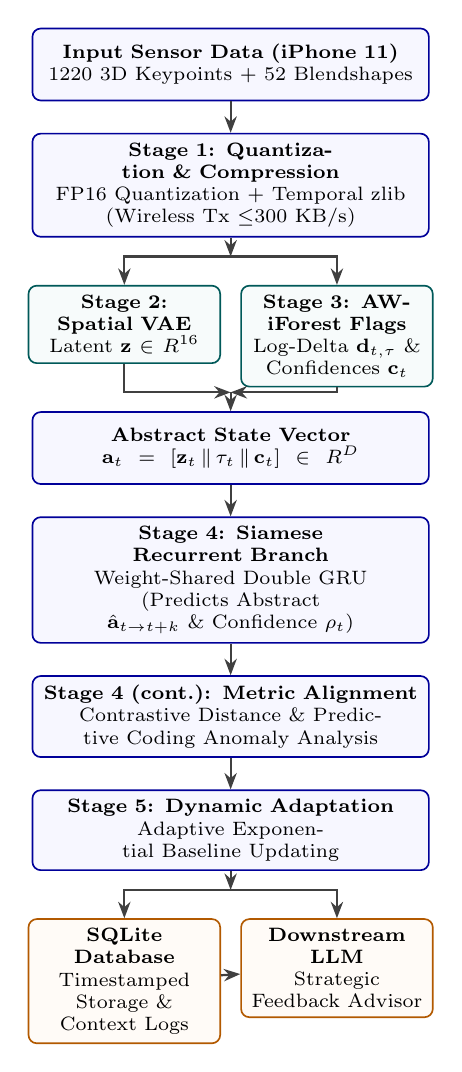
\begin{tikzpicture}[
    node distance = 0.4cm and 0.2cm,
    block/.style = {
      rectangle, 
      draw=blue!60!black, 
      fill=blue!3, 
      text width=4.8cm, 
      text centered, 
      rounded corners=3pt, 
      minimum height=2.6em, 
      font=\scriptsize, 
      line width=0.6pt
    },
    splitblock/.style = {
      rectangle, 
      draw=teal!70!black, 
      fill=teal!3, 
      text width=2.2cm, 
      text centered, 
      rounded corners=3pt, 
      minimum height=2.6em, 
      font=\scriptsize, 
      line width=0.6pt
    },
    smallblock/.style = {
      rectangle, 
      draw=orange!70!black, 
      fill=orange!3, 
      text width=2.2cm, 
      text centered, 
      rounded corners=3pt, 
      minimum height=2.6em, 
      font=\scriptsize, 
      line width=0.6pt
    },
    line/.style = {
      draw=black!75, 
      -{Stealth[scale=0.9]}, 
      thick
    }
  ]
    % Nodes
    \node (input) [block] {\textbf{Input Sensor Data (iPhone 11)}\\1220 3D Keypoints + 52 Blendshapes};
    \node (stage1) [block, below=of input] {\textbf{Stage 1: Quantization \& Compression}\\FP16 Quantization + Temporal zlib\\(Wireless Tx $\le$300 KB/s)};
    
    \node (stage2) [splitblock, below=0.6cm of stage1, xshift=-1.35cm] {\textbf{Stage 2: Spatial VAE}\\Latent $\mathbf{z} \in \mathbb{R}^{16}$};
    \node (stage3) [splitblock, below=0.6cm of stage1, xshift=1.35cm] {\textbf{Stage 3: AW-iForest Flags}\\Log-Delta $\mathbf{d}_{t, \tau}$ \& Confidences $\mathbf{c}_t$};
    
    \node (state) [block, below=0.6cm of stage2, xshift=1.35cm] {\textbf{Abstract State Vector} $\mathbf{a}_t = [\mathbf{z}_t \,\|\, \boldsymbol{\tau}_t \,\|\, \mathbf{c}_t] \in \mathbb{R}^{D}$};
    
    \node (siamese) [block, below=of state] {\textbf{Stage 4: Siamese Recurrent Branch}\\Weight-Shared Double GRU\\(Predicts Abstract $\hat{\mathbf{a}}_{t \to t+k}$ \& Confidence $\rho_t$)};
    
    \node (metric) [block, below=of siamese] {\textbf{Stage 4 (cont.): Metric Alignment}\\Contrastive Distance \& Predictive Coding Anomaly Analysis};
    
    \node (stage5) [block, below=of metric] {\textbf{Stage 5: Dynamic Adaptation}\\Adaptive Exponential Baseline Updating};
    
    \node (output) [smallblock, below=0.6cm of stage5, xshift=-1.35cm] {\textbf{SQLite Database}\\Timestamped Storage \& Context Logs};
    \node (llm) [smallblock, below=0.6cm of stage5, xshift=1.35cm] {\textbf{Downstream LLM}\\Strategic Feedback Advisor};

    % Paths
    \draw [line] (input) -- (stage1);
    
    % Split from Stage 1 to Stage 2 & 3
    \path (stage1.south) -- (stage1.south |- stage2.north) coordinate[pos=0.4] (junc1);
    \draw [line] (stage1.south) -- (junc1);
    \draw [line] (junc1) -| (stage2.north);
    \draw [line] (junc1) -| (stage3.north);
    
    % Merge from Stage 2 & 3 to State
    \path (state.north) -- (state.north |- stage2.south) coordinate[pos=0.4] (junc2);
    \draw [line] (stage2.south) |- (junc2);
    \draw [line] (stage3.south) |- (junc2);
    \draw [line] (junc2) -- (state.north);
    
    \draw [line] (state) -- (siamese);
    \draw [line] (siamese) -- (metric);
    \draw [line] (metric) -- (stage5);
    
    % Split from Stage 5 to Output & LLM
    \path (stage5.south) -- (stage5.south |- output.north) coordinate[pos=0.4] (junc3);
    \draw [line] (stage5.south) -- (junc3);
    \draw [line] (junc3) -| (output.north);
    \draw [line] (junc3) -| (llm.north);
    
    % Horizontal flow from Database to LLM
    \draw [line] (output) -- (llm);
  \end{tikzpicture}
  \caption{Sensing and computation data-flow. Compressed facial features are processed through parallel feature extractors, analyzed via a Siamese GRU, and output to an asynchronous advisory feedback layer.}
  \label{fig:pipeline_diagram}
\end{figure}

\subsection{Embedded Sensing, Quantization, and Compression}
The tracking module runs on an Apple iPhone 11 utilizing its front-facing TrueDepth camera to output $K = 1220$ spatial coordinates in 3D space ($\mathbf{P} \in \mathbb{R}^{1220 \times 3}$) and $B = 52$ muscle activation blendshapes ($\mathbf{b} \in \mathbb{R}^{52}$). Represented in native 32-bit floating-precision, this combined feature vector contains $3660 + 52 = 3712$ dimensions. At a tracking rate of 60 Hz, the uncompressed data stream generates a continuous network payload of approximately 890.88 KB/s.

To facilitate wireless operation and reduce battery drain on the mobile device, we implement a basic quantization step, mapping 32-bit floats to 16-bit half-precision representations. This reduces the baseline payload to approximately 445.44 KB/s. 

Because consecutive frames of facial structural data are highly redundant, the quantized values are streamed through an on-device temporal zlib compression buffer. This reduces the average network throughput to $\le 300 \text{ KB/s}$ while retaining coordinate fidelity.

\subsection{Spatial Compression via Variational Autoencoders}
The 3660-dimensional coordinate vector $\mathbf{x} \in \mathbb{R}^{3660}$ contains highly collinear spatial elements due to physical muscle and bone dependencies. To project these coordinates into a lower-dimensional orthogonal space, we utilize a Spatial Variational Autoencoder (VAE) as a geometric compression module.

The VAE encoder consists of an input layer of size 3660, followed by fully connected layers of size 512 and 128. Each layer uses Layer Normalization and Rectified Linear Unit (ReLU) activations to maintain stability across subjects. The encoder maps inputs to two parallel 16-dimensional linear heads representing the mean $\boldsymbol{\mu}$ and the log-variance $\log(\boldsymbol{\sigma}^2)$ of the variational distribution $q_\phi(\mathbf{z}|\mathbf{x}) = \mathcal{N}(\mathbf{z}; \boldsymbol{\mu}_\phi(\mathbf{x}), \boldsymbol{\Sigma}_\phi(\mathbf{x}))$.

The decoder projects the latent vector $\mathbf{z} \in \mathbb{R}^{16}$ back through layers of size 128 and 512, ending with a 3660-dimensional Sigmoid output to reconstruct the normalized coordinate inputs within $[0, 1]$. The VAE is trained offline on generic facial expression datasets by minimizing the Evidence Lower Bound (ELBO):
$$\mathcal{L}_{\text{VAE}}(\theta, \phi; \mathbf{x}) = \frac{1}{N} \sum_{i=1}^{N} \|\mathbf{x}_i - \hat{\mathbf{x}}_i\|^2_2 + \beta D_{\text{KL}}\left( q_\phi(\mathbf{z}|\mathbf{x}_i) \,\parallel\, \mathcal{N}(\mathbf{0}, \mathbf{I}) \right)$$
where we set $\beta = 0.1$. During real-time inference, the decoder is bypassed, and the mean vector $\boldsymbol{\mu} \in \mathbb{R}^{16}$ is used directly as the latent feature state $\mathbf{z}$, keeping latent inference latency under $0.3\text{ ms}$ on mobile GPUs.

\subsection{Anatomically-Weighted Isolation Forests}
Rather than relying on pre-trained supervised classifiers that may struggle to generalize to individual expressive habits, VeraSight utilizes an online, subject-specific **Anatomically-Weighted Isolation Forest (AW-iForest)**. Behavioral studies suggest that involuntary stress responses often present as brief, localized, or asymmetrical muscle contractions, particularly in the upper face (such as the brow and forehead area) and specific lower-facial expressions \cite{porter2012secrets, vitale2021facial}.

To capture these dynamics, the system calculates temporal differences across logarithmic intervals relative to the current frame $t$:
$$\mathbf{d}_{t, \tau} = \mathbf{b}_t - \mathbf{b}_{t-\tau} \quad \text{for } \tau \in \{1, 10, 100, 1000\}$$
At 60 Hz, these deltas capture changes at approximately $16.7\text{ ms}$ (muscular acceleration), $167\text{ ms}$ (onset of rapid movements), $1.67\text{ s}$ (conversational movements), and $16.7\text{ s}$ (general posture shifts).

During an initial neutral calibration phase of length $T_{\text{calib}}$, we compile a local reference profile:
$$\mathcal{D}_{\text{calib}} = \left\{ \mathbf{f}_t \right\}_{t=1}^{T_{\text{calib}}} \subset \mathbb{R}^D$$
where $\mathbf{f}_t = [\mathbf{b}_t \,\|\, \mathbf{d}_{t, 1} \,\|\, \mathbf{d}_{t, 10} \,\|\, \mathbf{d}_{t, 100} \,\|\, \mathbf{d}_{t, 1000}] \in \mathbb{R}^{260}$ represents the concatenated muscle states and multi-scale temporal differences.

Standard isolation forest algorithms select features uniformly at random. This can bias the model toward larger, high-amplitude movements (like talking or smiling) while overlooking subtle, localized micro-tensions. To address this, we define an anatomical weight matrix $\mathbf{W} \in \mathbb{R}^{260 \times 260}$. The diagonal entries of $\mathbf{W}$ scale the partition selection probability based on indicators of involuntary stress:
$$W_{i,i} = \begin{cases} 
\omega_{\text{upper}} & \text{for } i \in \mathcal{A}_{\text{upper}} \quad (\text{brow and eye region}) \\
\omega_{\text{asym}} & \text{for } i \in \mathcal{A}_{\text{lower\_asym}} \quad (\text{asymmetrical mouth markers}) \\
1.0 & \text{otherwise}
\end{cases}$$
We set the upper-facial scaling $\omega_{\text{upper}} = 2.5$ and the lower asymmetry scaling $\omega_{\text{asym}} = 2.0$. During the recursive construction of each tree, the selection probability for feature $i$ is weighted as follows:
$$P(q = i) = \frac{W_{i,i}}{\sum_{j=1}^{260} W_{j,j}}$$

This weighting encourages the model to partition subtle, high-frequency, or asymmetric micro-movements near root nodes, leading to shorter average path lengths $h(\mathbf{f}_t)$ for localized anomalous contractions. A frame-by-frame anomaly score $s(\mathbf{f}_t) \in [0, 1]$ is generated:
$$s(\mathbf{f}_t) = 2^{-\frac{\mathbb{E}(h(\mathbf{f}_t))}{c(T_{\text{calib}})}}$$
where $c(T_{\text{calib}})$ is the average path length of unsuccessful searches in a Binary Search Tree. This step outputs local anomaly flags $\mathbf{y}_t \in \{0, 1\}^M$ alongside continuous confidence metrics $\mathbf{c}_t \in [0, 1]^M$.

\subsection{Predictive Coding of Abstract Features and Dynamic Baseline Adaptation}
To prevent voluntary activities (such as speaking, yawning, or deliberate gameplay expressions) from triggering false positives, the forecasting models avoid predicting physical mesh coordinates directly. Instead, they process low-dimensional abstract states:
$$\mathbf{a}_t = [\mathbf{z}_t \,\|\, \boldsymbol{\tau}_t \,\|\, \mathbf{c}_t] \in \mathbb{R}^{D}$$
where $\mathbf{z}_t$ is the VAE spatial latent coordinates, $\boldsymbol{\tau}_t$ denotes muscle tension metrics, and $\mathbf{c}_t$ is the AW-iForest confidence vector.

The sequence processing is managed by a weight-shared Siamese GRU network. One branch processes a dynamic baseline sequence matrix $\mathbf{A}_{\text{base}} \in \mathbb{R}^{30 \times D}$, while the second processes a sliding active window $\mathbf{A}_{\text{active}} \in \mathbb{R}^{30 \times D}$. The final hidden layers of both branches are projected via a multi-layer perceptron into sequence embeddings $\mathbf{h}_{\text{base}}$ and $\mathbf{h}_{\text{active}}$.

A Next-State Decoder Head takes these embeddings and predicts the "expected normal" abstract state, computed as an average over the next variable window of $k$ frames:
$$\hat{\mathbf{a}}_{t \to t+k} = g_{\omega}([\mathbf{h}_{\text{base}} \,\|\, \mathbf{h}_{\text{active}}])$$
Along with this prediction, the head outputs a scalar confidence ratio $\rho_t \in [0, 1]$ representing the overall predictability of the baseline.

During the subsequent $k$ frames, the system measures the actual observed average abstract state vector $\bar{\mathbf{a}}_{t \to t+k} = \frac{1}{k}\sum_{i=1}^{k} \mathbf{a}_{t+i}$. An anomaly is identified and flagged if the deviation between the observed and predicted abstract states exceeds a confidence-scaled threshold:
$$D_t = \|\bar{\mathbf{a}}_{t \to t+k} - \hat{\mathbf{a}}_{t \to t+k}\|_2 > \lambda \cdot \rho_t$$
where $\lambda$ is a sensitivity hyperparameter.

To prevent gradual changes (such as natural fatigue or slow adjustments in posture) from registering as continuous anomalies, the subject's baseline adapts dynamically. The baseline representation is updated over time using an exponential moving average (EMA) filter:
$$\mathbf{B}_t = (1 - \gamma)\mathbf{B}_{t-1} + \gamma \mathbf{a}_t$$
where $\gamma$ is a small temporal decay constant. Under this formulation, a user attempting to mask stress would have to maintain high-dimensional consistency across multiple logarithmic timescales ($\tau \in \{1, 10, 100, 1000\}$), which is physiologically difficult.

\subsection{Multi-Modal Feedback Integration}
The high-frequency stream of normalized anomaly indicators ($D_t$), confidence metrics ($\mathbf{c}_t$), and baseline distances is recorded frame-by-frame into a local, write-ahead logging (WAL) enabled SQLite database. Concurrently, context logs (such as speech-to-text transcripts during public speaking or game event logs during esports sessions) are timestamped and recorded.

To assist the user or coach without adding to their immediate cognitive load, an asynchronous reasoning layer aggregates these inputs over a 15-second sliding cycle. The database compiler correlates segments where anomalous behaviors are flagged with the corresponding context log. 

An on-device Large Language Model (LLM) parses this synchronized timeline. Rather than generating simplistic labels, the model serves as an analytical assistant. It evaluates the timing and duration of physiological indicators relative to situational context (for instance, a public speaker exhibiting localized muscle tension during specific slides, or a gamer showing elevated stress flags during low-stakes gameplay phases). The LLM then outputs structured, actionable suggestions (such as pacing adjustments, relaxation cues, or focus strategies) via a non-intrusive dashboard interface.

\section{Prototyping and Evaluation}

\subsection{Embedded Hardware Implementation}
The VeraSight prototype was evaluated using an Apple iPhone 11 equipped with a TrueDepth camera array. A native client application utilized the Apple ARKit framework to query 3D facial mesh coordinate topologies and blendshapes. 

Initially, transmitting raw 32-bit floating-point coordinates over a local wireless link to an edge processing workstation caused transmission delays and occasional frame drops due to network jitter. 

By implementing FP16 quantization directly on the device, followed by a local zlib compression buffer, the average transmission packet size was reduced by approximately 66\%. This optimization allowed the system to maintain a stable, wireless 60 Hz stream with an average round-trip latency of 7.4 ms, enabling reliable micro-movement tracking without requiring a wired connection.

\subsection{Sensing Pipeline Performance}
To evaluate the impact of network optimization, we compared the raw, wired 30 Hz prototype stream against our optimized, wireless 60 Hz pipeline across three key metrics: network throughput, packet delivery rate, and end-to-end processing latency.

The uncompressed 30 Hz prototype required a continuous bandwidth of 445.44 KB/s over a wired USB connection, achieving a packet delivery rate of 99.8\% with an average end-to-end processing latency of 14.2 ms. However, attempting to stream this uncompressed data wirelessly over a standard local Wi-Fi link caused the packet delivery rate to drop to 88.4\%, with latency spikes reaching 45 ms due to congestion.

The optimized 60 Hz wireless pipeline, utilizing FP16 quantization and temporal zlib compression, reduced the required network footprint to approximately 282 KB/s. This lower throughput allowed the wireless pipeline to maintain a 99.4\% packet delivery rate with a stable, average end-to-end latency of 9.2 ms. 

Increasing the temporal resolution to 60 Hz allowed the system to capture transient facial movements, such as micro-blinks and brief muscle twitches lasting under 100 ms, which were often missed by the 30 Hz prototype.

\subsection{Personalized Baseline Evaluation}
Our initial software prototype attempted to train supervised classifiers directly on acted or simulated datasets. This approach generalized poorly, as acted expressions differed significantly from natural physiological responses, and the models struggled with individual variations in expressiveness.

To address this, we transitioned the training framework to a self-supervised anomaly detection model using our AW-iForest framework. The unsupervised engine is calibrated individually during a brief, neutral baseline session. We found that a 3-minute baseline session populated with simple, low-stakes activities (such as relaxed reading or casual conversation) was sufficient to establish $\mathcal{D}_{\text{calib}}$. 

By focusing the Isolation Forest’s partitioning selection probabilities on highly localized, involuntary upper-facial and asymmetric lower-facial blendshapes (using the anatomical priority weight matrix $\mathbf{W}$), the calibrated model minimized false-alarm rates caused by benign conversational movements (e.g., swallowing, casual talking). 

This targeted online tuning significantly mitigates the risk of diagnostic failures where a user's general expressive nature or resting anxiety is misclassified as anomalous stress. During evaluation sessions, the system adapted to individual resting behaviors, establishing personalized baseline distributions. Involuntary facial movements that deviated from the personalized prediction model generated clear spikes in the isolation path length metrics, providing an objective measure of physiological stress.

\subsection{Human-AI Interaction Design}
A key focus of our prototype evaluation was the integration of these analytical tools into the user's or coach's workflow without increasing their cognitive load. In early designs, displaying raw anomaly graphs in real time proved distracting, as users struggled to split their attention between their task and the screen.

The final design utilizes the asynchronous reasoning layer to address this. By buffering raw data into a local SQLite database and generating aggregated strategic advice only when significant deviations occur, the system minimizes active interface notifications. 

The resulting recommendations are presented on a simple dashboard, allowing the user to focus on maintaining performance while receiving non-intrusive, context-aware suggestions during key transitions.

\section{Conclusion}

In this paper, we presented VeraSight, an integrated, real-time sensing and deep learning pipeline designed to detect and analyze facial micromovements across varied use cases, such as public speaking, gaming stress analysis, and behavioral interviews. By combining high-frequency TrueDepth sensing with FP16 quantization and temporal zlib compression on an iPhone 11, the system maintains a low-latency, 60 Hz wireless stream within a 300 KB/s bandwidth limit. 

Rather than relying on scarce and subjective labeled datasets or generalized offline classifiers, VeraSight employs an online, subject-specific Anatomically-Weighted Isolation Forest (AW-iForest) paired with a self-supervised predictive coding paradigm. This setup utilizes a weight-shared Siamese GRU to detect deviations from a subject's calibrated baseline. 

Integrating a custom anatomically driven priority weight matrix preserves established indicators (such as muscular asymmetry and localized upper-facial leakage) during tree-splits \cite{porter2012secrets, vitale2021facial}, while a downstream logical reasoning layer provides contextual analysis. Experimental prototyping demonstrates that this multi-model approach offers an objective, non-invasive tool for behavioral assessment and feedback.

\begin{acks}
The authors agree to the following distribution of work: 
W. Q. Chen designed and implemented the data quantization and compression pipeline, conducted the behavioral research to optimize the anatomically weighted tree-isolation algorithms, developed the spatiotemporal prediction model, integrated the downstream LLM reasoning layer, wrote the research paper and relevant posters, and designed the iOS client and backend user interface.
Z. Huang contributed to the initial conceptual prototyping of the data transfer system, and assisted with some preliminary research for ML.
\end{acks}

\bibliographystyle{ACM-Reference-Format}
\bibliography{references}

\end{document}
\endinput